%% abtex2-modelo-trabalho-academico.tex, laurocesar
%% Copyright 2012-2015 by abnTeX2 group at http://www.abntex.net.br/ 
%%
%% This work may be distributed and/or modified under the
%% conditions of the LaTeX Project Public License, either version 1.3
%% of this license or (at your option) any later version.
%% The latest version of this license is in
%%   http://www.latex-project.org/lppl.txt
%% and version 1.3 or later is part of all distributions of LaTeX
%% version 2005/12/01 or later.
%%
%% This work has the LPPL maintenance status `maintained'.
%% 
%% The Current Maintainer of this work is the abnTeX2 team, led
%% by Lauro César Araujo. Further information are available on 
%% http://www.abntex.net.br/
%%
%% This work consists of the files abntex2-modelo-trabalho-academico.tex,
%% abntex2-modelo-include-comandos and abntex2-modelo-references.bib
%%

% ------------------------------------------------------------------------
% ------------------------------------------------------------------------
% abnTeX2: Modelo de Trabalho Academico (tese de doutorado, dissertacao de
% mestrado e trabalhos monograficos em geral) em conformidade com 
% ABNT NBR 14724:2011: Informacao e documentacao - Trabalhos academicos -
% Apresentacao
% ------------------------------------------------------------------------
% ------------------------------------------------------------------------

\documentclass[
	% -- opções da classe memoir --
	12pt,				% tamanho da fonte
	openright,			% capítulos começam em pág ímpar (insere página vazia caso preciso)
	oneside,			% para impressão em verso e anverso. Oposto a oneside
	a4paper,			% tamanho do papel. 
	% -- opções da classe abntex2 --
	chapter=TITLE,		% títulos de capítulos convertidos em letras maiúsculas
	%section=TITLE,		% títulos de seções convertidos em letras maiúsculas
	%subsection=TITLE,	% títulos de subseções convertidos em letras maiúsculas
	%subsubsection=TITLE,% títulos de subsubseções convertidos em letras maiúsculas
	% -- opções do pacote babel --
	english,			% idioma adicional para hifenização
	french,				% idioma adicional para hifenização
	spanish,			% idioma adicional para hifenização
	brazil				% o último idioma é o principal do documento
	]{abntex2}

% ---
% Pacotes básicos 
% ---
\usepackage{helvet}			% Usa a fonte Latin Modern - Mudei para Helvetica
\usepackage[T1]{fontenc}		% Selecao de codigos de fonte.
\usepackage[utf8]{inputenc}	% Codificacao do documento (conversão automática dos acentos)
\usepackage{lastpage}		% Usado pela Ficha catalográfica
\usepackage{indentfirst}		% Indenta o primeiro parágrafo de cada seção.
\usepackage{color}			% Controle das cores
\usepackage{graphicx}		% Inclusão de gráficos
\usepackage{microtype} 		% para melhorias de justificação
% ---
		
% ---
% Pacotes adicionais, usados apenas no âmbito do Modelo Canônico do abnteX2
% ---
\usepackage{lipsum}				% para geração de dummy text
\usepackage{customizacoes} 		% customizações feitas pelo autor
% ---

% ---
% Pacotes de citações
% ---
\usepackage[brazilian,hyperpageref]{backref}	% Paginas com as citações na bibl
\usepackage[alf]{abntex2cite}				% Citações padrão ABNT

% --- 
% CONFIGURAÇÕES DE PACOTES
% --- 

% ---
% Configurações do pacote backref
% Usado sem a opção hyperpageref de backref
\renewcommand{\backrefpagesname}{ }
% Texto padrão antes do número das páginas
\renewcommand{\backref}{\ABNTEXchapterfont}
% Define os textos da citação
\renewcommand*{\backrefalt}[4]{
	\ifcase #1 %
		%
	\or
		%
	\else
		%
	\fi}%
% ---

% ---
% Informações de dados para CAPA e FOLHA DE ROSTO
% ---
\titulo{Habilitando um Prédio a Localizar Contextualmente Dispositivos utilizando Redes Sem Fio}
\autor{Luís Henrique Puhl de Souza}
\local{Bauru}
\data{2016}
\orientador{Prof. Dr. Eduardo Martins Morgado}

\instituicao{%
  Universidade Estadual Paulista "Júlio de Mesquita Filho"
  %\par
  Faculdade de Ciências - Campus Bauru
  %\par
  Departamento de Computação
}
\tipotrabalho{Monografia (Trabalho de Conclusão de Curso)}
% O preambulo deve conter o tipo do trabalho, o objetivo, 
% o nome da instituição e a área de concentração 
\preambulo{Projeto de Trabalho de Conclusão de Curso de Bacharelado em Ciência da Computação da Universidade Estadual Paulista "Júlio de Mesquita Filho", Faculdade de Ciências, campus Bauru
	}
% ---

% ---
% Configurações de projeto
% --- 
\newif\iffinal
\finalfalse % define se é um arquivo final, se for não for retira umas partes. 

\newif\ifabstract
\abstractfalse % define se mostra o abstract em inglês ou não.

% --- 


% ---
% Configurações de aparência do PDF final

% alterando o aspecto da cor azul
\definecolor{blue}{RGB}{0,0,0}

% informações do PDF
\makeatletter
\hypersetup{
     	%pagebackref=true,
		pdftitle={\@title}, 
		pdfauthor={\@author},
    	pdfsubject={\imprimirpreambulo},
	    pdfcreator={LaTeX with abnTeX2},
		pdfkeywords={beacon}{raspberry pi}{internet das coisas}{abntex2}{trabalho acadêmico}, 
		colorlinks=true,       		% false: boxed links; true: colored links
    	linkcolor=blue,          	% color of internal links
    	citecolor=blue,        		% color of links to bibliography
    	filecolor=magenta,      		% color of file links
		urlcolor=blue,
		bookmarksdepth=4
}
\makeatother
% --- 

% --- 
% Espaçamentos entre linhas e parágrafos 
% --- 

% O tamanho do parágrafo é dado por:
\setlength{\parindent}{1.3cm}

% Controle do espaçamento entre um parágrafo e outro:
\setlength{\parskip}{0.2cm}  % tente também \onelineskip

% ---
% compila o indice
% ---
\makeindex
% ---

% ----
% Início do documento
% ----
\begin{document}

% Seleciona o idioma do documento (conforme pacotes do babel)
%\selectlanguage{english}
\selectlanguage{brazil}

% Retira espaço extra obsoleto entre as frases.
\frenchspacing 

% ----------------------------------------------------------
% ELEMENTOS PRÉ-TEXTUAIS
% ----------------------------------------------------------
\pretextual

\ABNTEXchapterfont {

% ---
% Capa
% ---
\imprimircapa
% ---

% ---
% Folha de rosto
% (o * indica que haverá a ficha bibliográfica)
% ---
%\imprimirfolhaderosto
% ---

% ---
% Inserir a ficha bibliografica
% ---

% Isto é um exemplo de Ficha Catalográfica, ou ``Dados internacionais de
% catalogação-na-publicação''. Você pode utilizar este modelo como referência. 
% Porém, provavelmente a biblioteca da sua universidade lhe fornecerá um PDF
% com a ficha catalográfica definitiva após a defesa do trabalho. Quando estiver
% com o documento, salve-o como PDF no diretório do seu projeto e substitua todo
% o conteúdo de implementação deste arquivo pelo comando abaixo:
%
% \begin{fichacatalografica}
%     \includepdf{fig_ficha_catalografica.pdf}
% \end{fichacatalografica}

\iffinal
  \begin{fichacatalografica}
	\sffamily
	\vspace*{\fill}					% Posição vertical
	\begin{center}					% Minipage Centralizado
	\fbox{\begin{minipage}[c][8cm]{13.5cm}		% Largura
	\small
	\imprimirautor
	%Sobrenome, Nome do autor
	
	\hspace{0.5cm} \imprimirtitulo  / \imprimirautor. --
	\imprimirlocal, \imprimirdata-
	
	\hspace{0.5cm} \pageref{LastPage} p. : il. (algumas color.) ; 30 cm.\\
	
	\hspace{0.5cm} \imprimirorientadorRotulo~\imprimirorientador\\
	
	\hspace{0.5cm}
	\parbox[t]{\textwidth}{\imprimirtipotrabalho~--~\\ \imprimirinstituicao,
	\imprimirdata.}\\
	
	\hspace{0.5cm}
		1. Beacon.
		2. Raspberry Pi.
		2. Internet das Coisas.
		I. \imprimirorientador.
		II. Universidade Estadual Paulista "Júlio de Mesquita Filho".
		III. Faculdade de Ciências.
		IV. Título
	\end{minipage}}
	\end{center}
  \end{fichacatalografica}
\fi
% ---

% ---
% Inserir errata
% ---
%\begin{errata}
%Elemento opcional da \citeonline[4.2.1.2]{NBR14724:2011}. Exemplo:

%\vspace{\onelineskip}

%FERRIGNO, C. R. A. \textbf{Tratamento de neoplasias ósseas apendiculares com
%reimplantação de enxerto ósseo autólogo autoclavado associado ao plasma
%rico em plaquetas}: estudo crítico na cirurgia de preservação de membro em
%cães. 2011. 128 f. Tese (Livre-Docência) - Faculdade de Medicina Veterinária e
%Zootecnia, Universidade de São Paulo, São Paulo, 2011.

%\begin{table}[htb]
%\center
%\footnotesize
%\begin{tabular}{|p{1.4cm}|p{1cm}|p{3cm}|p{3cm}|}
%  \hline
%   \textbf{Folha} & \textbf{Linha}  & \textbf{Onde se lê}  & \textbf{Leia-se}  \\
%    \hline
%    1 & 10 & auto-conclavo & autoconclavo\\
%   \hline
%\end{tabular}
%\end{table}

%\end{errata}
% ---

% ---
% Inserir folha de aprovação
% ---

% Isto é um exemplo de Folha de aprovação, elemento obrigatório da NBR
% 14724/2011 (seção 4.2.1.3). Você pode utilizar este modelo até a aprovação
% do trabalho. Após isso, substitua todo o conteúdo deste arquivo por uma
% imagem da página assinada pela banca com o comando abaixo:
%
% \includepdf{folhadeaprovacao_final.pdf}
%
\begin{folhadeaprovacao}
  \ABNTEXchapterfont {

    \begin{center}
    
      {\ImprimirAutor}

      \vspace*{\fill}\vspace*{\fill}
      
      \begin{center}
        \bfseries\large\ImprimirTitulo
      \end{center}
      
      \vspace*{\fill}
    
      \hspace{.45\textwidth}
      \begin{minipage}{.5\textwidth}
          \imprimirpreambulo
      \end{minipage}%
      \vspace*{\fill}
     \end{center}
        
     %Trabalho aprovado. \imprimirlocal, 24 de novembro de 2012:

     %\assinatura{\textbf{\imprimirorientador} \\ Orientador}
     %\assinatura{\textbf{\imprimircoorientador} \\ Coorientador} 
     %\assinatura{\textbf{Professor} \\ Convidado 1}
     %\assinatura{\textbf{Professor} \\ Convidado 2}
     %\assinatura{\textbf{Professor} \\ Convidado 3}
     %\assinatura{\textbf{Professor} \\ Convidado 4}
      \vspace*{0.5cm}
      \hspace{.5\textwidth}
     \begin{center} 
       \ImprimirLocal \\ \imprimirdata
     \end{center}
  }
\end{folhadeaprovacao}
% ---

% ---
% Dedicatória
% ---
\iffinal
  \begin{dedicatoria} 
   \vspace*{\fill}
   \centering
   \noindent
   \textit{} \vspace*{\fill}
  \end{dedicatoria}
\fi
% ---

% ---
% Agradecimentos
% ---
\iffinal
  \begin{agradecimentos}


\end{agradecimentos}
\fi
% ---

% ---
% Epígrafe
% ---
\iffinal
  \begin{epigrafe}
    \vspace*{\fill}
	\begin{flushright}
		\textit{}
	\end{flushright}
  \end{epigrafe}
\fi
% ---

% ---
% RESUMOS
% ---
\ifabstract
% resumo em português
\setlength{\absparsep}{18pt} % ajusta o espaçamento dos parágrafos do resumo
\begin{resumo}
\ABNTEXchapterfont {
 
 \textbf{Palavras-chave}: \textit{Redes Neurais Artificiais}. Cloud Computing. Balanceamento de Carga.
}
\end{resumo}

% resumo em inglês
\begin{resumo}[Abstract]
 \begin{otherlanguage*}{english}
   This is the english abstract.

   \vspace{\onelineskip}
 
   \noindent 
   \textbf{Keywords}: Artificial Neural Networks. Cloud Computing. Load Balancing.
 \end{otherlanguage*}
\end{resumo}
\fi
% ---

% ---
% inserir lista de ilustrações
% ---
\iffinal
  \pdfbookmark[0]{\listfigurename}{lof}
  \listoffigures*
  \cleardoublepage
\fi
% ---

% ---
% inserir lista de tabelas
% ---
\iffinal
  \pdfbookmark[0]{\listtablename}{lot}
  \listoftables*
  \cleardoublepage
\fi
% ---

% ---
% inserir lista de abreviaturas e siglas
% ---
\iffinal
  \begin{siglas}
    \item[ANN] \textit{Artificial Neural Networks}    
  \end{siglas}
\fi
% ---

% ---
% inserir lista de símbolos
% ---
\iffinal
  \begin{simbolos}
    \item[$ \Gamma $] Letra grega Gama
    \item[$ \Lambda $] Lambda
    \item[$ \zeta $] Letra grega minúscula zeta
    \item[$ \in $] Pertence
  \end{simbolos}
\fi
% ---

% ---
% inserir o sumario
% ---
\pdfbookmark[0]{\contentsname}{toc}
\tableofcontents*
\cleardoublepage
% ---






% ----------------------------------------------------------------------------------------------------------------------------------
% ELEMENTOS TEXTUAIS
% ----------------------------------------------------------------------------------------------------------------------------------
\textual

% ---
% Introdução
% ---
\chapter[Introdução]{Introdução}
%\addcontentsline{toc}{chapter}{Introdução}
% ----------------------------------------------------------
Recentemente IoT (\textit{Internet of Things} - Internet das Coisas) vem tomando o foco das atenções de empresas e entusiastas de IT (\textit{Information Tecnology} - Tecnologia da Informação) \cite{DzoneIoT:2015}a tal ponto que, as empresas líderes do segmento já incluem IoT como um de seus segmentos \cite{Ibm2016} \cite{ARM} \cite{Microsoft2016} \cite{Intel2016} \cite{Oracle2016} \cite{Google2016} \cite{AmazonIoT2016}.

Todo este movimento no mercado é justificado pelo baixo custo de dispositivos \cite{Raspberryfundation2012} \cite{Esp8266.net} e serviços \cite{Kaufmann2015} \cite{Amazon2016}. Este baixo custo possibilita a computação ubíqua [Weiser 1991] que é entendida pelos autores como "computação virtualmente onipresente". Também para os autores, esta virtual onipresença é base e consequência para a IoT, levando à visão de que a mesma [IoT] como realizadora da computação ubíqua.

Uma vez contextualizado o mercado e a oportunidade de implementação da computação ubíqua, percebemos a necessidade de dar aos elementos cotidianos (coisas) a capacidade info-computacional, tornando-os sensores e atuadores conectados, unicamente identificáveis e acessíveis através da rede mundial (internet) \cite{Lemos2013} \cite{Kranenburg2012}.

É esperado que estas coisas conectadas (dispositivos) até o final de 2016 representem uma quantia total de 6,4 bilhões \cite{GARTNER2016}.


% ---

% ---
% Problema
% ---
\chapter{Problema}
% ---
A grande quantidade de dispositivos traz o desafio de localizá-los contextualmente, tanto para (1) que o dispositivo tome ciência de sua posição em um contexto além de sua posição global em suas tomadas de decisão e (2) para que outros (sistemas, pessoas e coisas) saibam a localização de qualquer dispositivo ao qual tem interesse de interagir.

Mesmo com a grande quantidade de dispositivos já conectados são poucos os documentos descrevendo boas práticas para concepção, construção e manutenção de aplicações IoT, especialmente sobre os cuidados tomados quanto a segurança e análise de custos para a implementação e manutenção. Além disso, a falta de referências neste sentido é agravada quando considera-se implementação no interior do estado de São Paulo.


% ---

% ---
% Justificativa
% ---
\chapter{Justificativa}
% ---
Na visão dos autores, promover o desenvolvimento local através de trabalhos exemplo, treinamentos ou manuais é fundamental para a equiparação dos desenvolvedores locais com as tecnologias e tendencias de mercado então justificamos sua execução para que outras organizações possam encontrar novos caminhos.

% ---

% ---
% Objetivos
% ---
\chapter{Objetivos}
% ---

% ---

% ---
\section{Objetivos Gerais}
% ---
Considerando características locais, propõem-se a construção de uma aplicação para localizar contextualmente dispositivos dentro de um prédio piloto e avaliar sua precisão.

Além desta aplicação, é objetivo definir o custo do projeto piloto incluindo esforço de pesquisa assim como definir um custo para replicação deste localizador contextual em outros prédios.

% ---

% ---
\section{Objetivos Específicos}
% ---

\begin{alineas}
	\item Estabelecer o estado da arte sobre a desenvolvimento de aplicações IoT;
	\item Identificar desafios locais para o desenvolvimento;
	\item Identificar provedores de serviços, dispositivos e ferramentas para o desenvolvimento;
	\item Construir um protótipo de sala conectada virtualmente que identifique os dispositivos conectados a rede que existem dentro nela através de conexões sem fio;
	\item Estimar o custo total do projeto piloto incluindo esforço de pesquisa;
	\item Estimar o custo de replicação da aplicação em outros prédios.
\end{alineas}

% ---

% ---
% Método de Pesquisa
% ---
\chapter{Método de Pesquisa}
% ---

Utilizaremos prototipagem ágil semelhante ao desenvolvimento de um produto utilizando a metodologia \textit{Scrum} \cite{James2016}, executando iterações de uma semana onde a cada iteração uma nova versão melhorada do produto completo (hardware, software, documentação e resultados) será entregue.

Dentro de cada iteração as camadas da aplicação IoT serão escolhidas, implementadas, justificadas e avaliadas sendo todo processo documentado. Como resultado de cada iteração será gerado um relatório das mudanças a partir da iteração anterior.

\begin{figure}[htb]
	\caption{\label{fig:projeto}Modelo das camadas }
	\begin{center}
		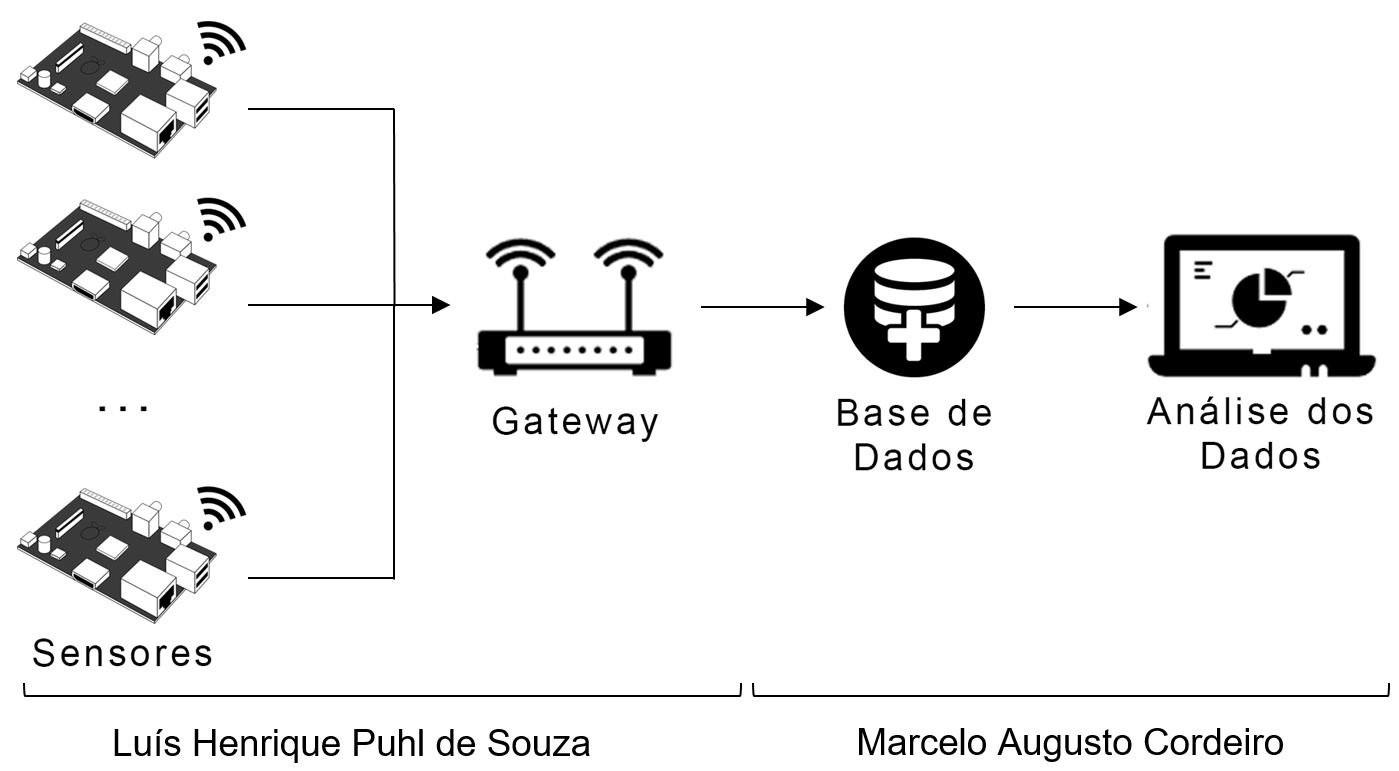
\includegraphics[width=1\textwidth]{img/projeto.JPG}
	\end{center}
	\legend{Fonte: Marcelo Augusto Cordeiro}
\end{figure}

A Figura \ref{fig:projeto} apresenta a arquitetura simplificada de uma aplicação IoT. Esta será modificada a cada iteração do projeto especialmente as camadas de sensores, \textit{gateway} e base de dados.


% ---

% ---
% Fundamentação Teórica
% ---
%\chapter{Fundamentação Teórica}
% ---

%Precisa? 

% ---

% ---
% Cronograma
% ---
\chapter{Cronograma}
% ---


Devido a natureza ágil e iterativa da metodologia, o cronograma será dividido em apenas três partes: Levantamento Bibliográfico Inicial, Desenvolvimento Iterativo e Revisão Final. Estas partes serão distribuídas conforme a Tabela~\ref{table:cronograma}.

\begin{table}[htb]
\IBGEtab{%
\ABNTEXchapterfont {
  \caption{Cronograma de Atividades Propostas}%
  \label{table:cronograma}
}
}{%
  \begin{tabular}{cccccccccc}
  \toprule
   Atividade							&	Fev	&	Mar	&	Abr	&	Mai	&	Jun	&	Jul	&	Ago	&	Set	&	Out \\
  \midrule \midrule
   Levantamento Bibliográfico Inicial	&	X	&	X	&	 	&	 	&	 	&	 	&	 	&	 	&	  \\
  \midrule 
  Desenvolvimento Iterativo				&	 	&	X	&	X	&	X	&	X	&	X	&	X	&	X	&	  \\
  \midrule 
  Revisão Final							&	 	&	 	&	 	&	 	&	 	&	 	&	 	&	X	&	X \\
  \bottomrule
\end{tabular}%
}{%
  \fonte{Produzido pelo autor.}%
  }
\end{table}

% ---


% ---
% Conclusão
% ---
%\chapter{Conclusão}
% ---

%\lipsum[1]

% ---


% ----------------------------------------------------------------------------------------------------------------------------------






% ----------------------------------------------------------
% ELEMENTOS PÓS-TEXTUAIS
% ----------------------------------------------------------

% ----------------------------------------------------------

% ----------------------------------------------------------
% Referências bibliográficas
% ----------------------------------------------------------
\bibliography{referencias}

}
\end{document}